% Options for packages loaded elsewhere
\PassOptionsToPackage{unicode}{hyperref}
\PassOptionsToPackage{hyphens}{url}
%
\documentclass[
]{article}
\usepackage{amsmath,amssymb}
\usepackage{iftex}
\ifPDFTeX
  \usepackage[T1]{fontenc}
  \usepackage[utf8]{inputenc}
  \usepackage{textcomp} % provide euro and other symbols
\else % if luatex or xetex
  \usepackage{unicode-math} % this also loads fontspec
  \defaultfontfeatures{Scale=MatchLowercase}
  \defaultfontfeatures[\rmfamily]{Ligatures=TeX,Scale=1}
\fi
\usepackage{lmodern}
\ifPDFTeX\else
  % xetex/luatex font selection
\fi
% Use upquote if available, for straight quotes in verbatim environments
\IfFileExists{upquote.sty}{\usepackage{upquote}}{}
\IfFileExists{microtype.sty}{% use microtype if available
  \usepackage[]{microtype}
  \UseMicrotypeSet[protrusion]{basicmath} % disable protrusion for tt fonts
}{}
\makeatletter
\@ifundefined{KOMAClassName}{% if non-KOMA class
  \IfFileExists{parskip.sty}{%
    \usepackage{parskip}
  }{% else
    \setlength{\parindent}{0pt}
    \setlength{\parskip}{6pt plus 2pt minus 1pt}}
}{% if KOMA class
  \KOMAoptions{parskip=half}}
\makeatother
\usepackage{xcolor}
\usepackage[margin=1in]{geometry}
\usepackage{color}
\usepackage{fancyvrb}
\newcommand{\VerbBar}{|}
\newcommand{\VERB}{\Verb[commandchars=\\\{\}]}
\DefineVerbatimEnvironment{Highlighting}{Verbatim}{commandchars=\\\{\}}
% Add ',fontsize=\small' for more characters per line
\usepackage{framed}
\definecolor{shadecolor}{RGB}{248,248,248}
\newenvironment{Shaded}{\begin{snugshade}}{\end{snugshade}}
\newcommand{\AlertTok}[1]{\textcolor[rgb]{0.94,0.16,0.16}{#1}}
\newcommand{\AnnotationTok}[1]{\textcolor[rgb]{0.56,0.35,0.01}{\textbf{\textit{#1}}}}
\newcommand{\AttributeTok}[1]{\textcolor[rgb]{0.13,0.29,0.53}{#1}}
\newcommand{\BaseNTok}[1]{\textcolor[rgb]{0.00,0.00,0.81}{#1}}
\newcommand{\BuiltInTok}[1]{#1}
\newcommand{\CharTok}[1]{\textcolor[rgb]{0.31,0.60,0.02}{#1}}
\newcommand{\CommentTok}[1]{\textcolor[rgb]{0.56,0.35,0.01}{\textit{#1}}}
\newcommand{\CommentVarTok}[1]{\textcolor[rgb]{0.56,0.35,0.01}{\textbf{\textit{#1}}}}
\newcommand{\ConstantTok}[1]{\textcolor[rgb]{0.56,0.35,0.01}{#1}}
\newcommand{\ControlFlowTok}[1]{\textcolor[rgb]{0.13,0.29,0.53}{\textbf{#1}}}
\newcommand{\DataTypeTok}[1]{\textcolor[rgb]{0.13,0.29,0.53}{#1}}
\newcommand{\DecValTok}[1]{\textcolor[rgb]{0.00,0.00,0.81}{#1}}
\newcommand{\DocumentationTok}[1]{\textcolor[rgb]{0.56,0.35,0.01}{\textbf{\textit{#1}}}}
\newcommand{\ErrorTok}[1]{\textcolor[rgb]{0.64,0.00,0.00}{\textbf{#1}}}
\newcommand{\ExtensionTok}[1]{#1}
\newcommand{\FloatTok}[1]{\textcolor[rgb]{0.00,0.00,0.81}{#1}}
\newcommand{\FunctionTok}[1]{\textcolor[rgb]{0.13,0.29,0.53}{\textbf{#1}}}
\newcommand{\ImportTok}[1]{#1}
\newcommand{\InformationTok}[1]{\textcolor[rgb]{0.56,0.35,0.01}{\textbf{\textit{#1}}}}
\newcommand{\KeywordTok}[1]{\textcolor[rgb]{0.13,0.29,0.53}{\textbf{#1}}}
\newcommand{\NormalTok}[1]{#1}
\newcommand{\OperatorTok}[1]{\textcolor[rgb]{0.81,0.36,0.00}{\textbf{#1}}}
\newcommand{\OtherTok}[1]{\textcolor[rgb]{0.56,0.35,0.01}{#1}}
\newcommand{\PreprocessorTok}[1]{\textcolor[rgb]{0.56,0.35,0.01}{\textit{#1}}}
\newcommand{\RegionMarkerTok}[1]{#1}
\newcommand{\SpecialCharTok}[1]{\textcolor[rgb]{0.81,0.36,0.00}{\textbf{#1}}}
\newcommand{\SpecialStringTok}[1]{\textcolor[rgb]{0.31,0.60,0.02}{#1}}
\newcommand{\StringTok}[1]{\textcolor[rgb]{0.31,0.60,0.02}{#1}}
\newcommand{\VariableTok}[1]{\textcolor[rgb]{0.00,0.00,0.00}{#1}}
\newcommand{\VerbatimStringTok}[1]{\textcolor[rgb]{0.31,0.60,0.02}{#1}}
\newcommand{\WarningTok}[1]{\textcolor[rgb]{0.56,0.35,0.01}{\textbf{\textit{#1}}}}
\usepackage{graphicx}
\makeatletter
\def\maxwidth{\ifdim\Gin@nat@width>\linewidth\linewidth\else\Gin@nat@width\fi}
\def\maxheight{\ifdim\Gin@nat@height>\textheight\textheight\else\Gin@nat@height\fi}
\makeatother
% Scale images if necessary, so that they will not overflow the page
% margins by default, and it is still possible to overwrite the defaults
% using explicit options in \includegraphics[width, height, ...]{}
\setkeys{Gin}{width=\maxwidth,height=\maxheight,keepaspectratio}
% Set default figure placement to htbp
\makeatletter
\def\fps@figure{htbp}
\makeatother
\setlength{\emergencystretch}{3em} % prevent overfull lines
\providecommand{\tightlist}{%
  \setlength{\itemsep}{0pt}\setlength{\parskip}{0pt}}
\setcounter{secnumdepth}{-\maxdimen} % remove section numbering
\ifLuaTeX
  \usepackage{selnolig}  % disable illegal ligatures
\fi
\IfFileExists{bookmark.sty}{\usepackage{bookmark}}{\usepackage{hyperref}}
\IfFileExists{xurl.sty}{\usepackage{xurl}}{} % add URL line breaks if available
\urlstyle{same}
\hypersetup{
  pdftitle={Exercise 1},
  pdfauthor={Adam Sulak, Onder Akacik, Arda Ergin},
  hidelinks,
  pdfcreator={LaTeX via pandoc}}

\title{Exercise 1}
\author{Adam Sulak, Onder Akacik, Arda Ergin}
\date{2024-02-22}

\begin{document}
\maketitle

\begin{Shaded}
\begin{Highlighting}[]
\FunctionTok{library}\NormalTok{(ggplot2)}
\FunctionTok{library}\NormalTok{(lme4)}
\end{Highlighting}
\end{Shaded}

\begin{verbatim}
## Loading required package: Matrix
\end{verbatim}

\hypertarget{exercise-1}{%
\section{Exercise 1}\label{exercise-1}}

\hypertarget{question-1a}{%
\subsection{Question 1a)}\label{question-1a}}

After loading \texttt{Ice\_cream-1.csv}, we first check the
\textbf{``normality assumption''}. The Normal QQ-plot, density plot, and
the histogram indicate that there does not seem to be a serious
deviation from normal distribution. The box plot indicate that there
seems to be no serious outliers.

\begin{Shaded}
\begin{Highlighting}[]
\FunctionTok{par}\NormalTok{(}\AttributeTok{mfrow =} \FunctionTok{c}\NormalTok{(}\DecValTok{1}\NormalTok{,}\DecValTok{2}\NormalTok{))}
\FunctionTok{hist}\NormalTok{(data}\SpecialCharTok{$}\NormalTok{video,}\AttributeTok{main =} \StringTok{"Histogram of Video Game Scores"}\NormalTok{, }\AttributeTok{xlab =} \StringTok{"Video Game Scores"}\NormalTok{)}
\FunctionTok{qqnorm}\NormalTok{(data}\SpecialCharTok{$}\NormalTok{video)}
\end{Highlighting}
\end{Shaded}

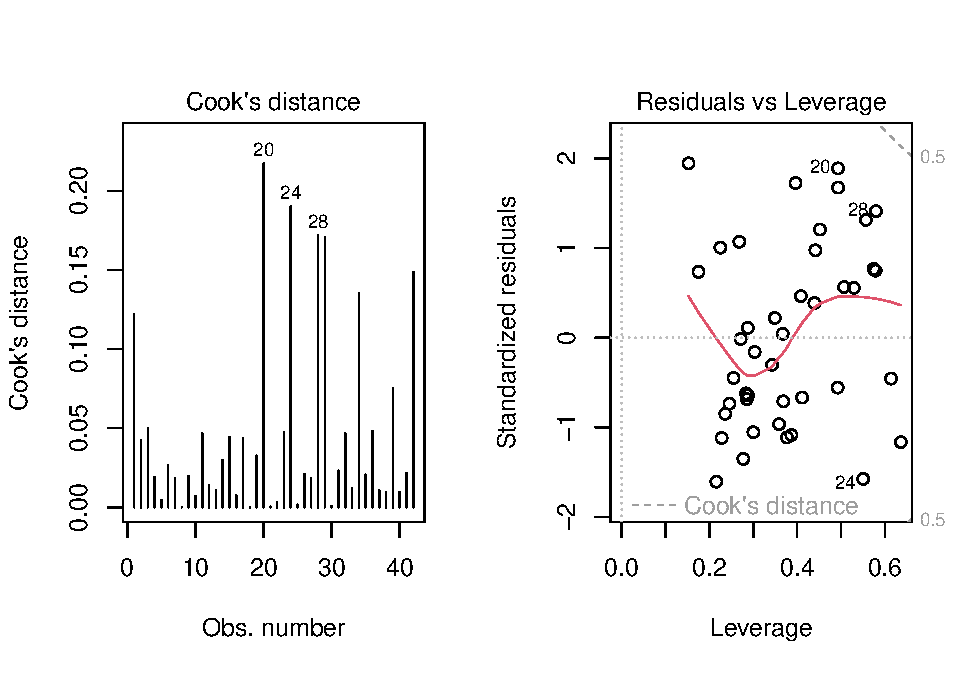
\includegraphics{Exercise-1_files/figure-latex/unnamed-chunk-3-1.pdf}

\begin{Shaded}
\begin{Highlighting}[]
\FunctionTok{par}\NormalTok{(}\AttributeTok{mfrow =} \FunctionTok{c}\NormalTok{(}\DecValTok{1}\NormalTok{,}\DecValTok{2}\NormalTok{))}
\FunctionTok{boxplot}\NormalTok{(data}\SpecialCharTok{$}\NormalTok{video); }\FunctionTok{plot}\NormalTok{(}\FunctionTok{density}\NormalTok{(data}\SpecialCharTok{$}\NormalTok{video))}
\end{Highlighting}
\end{Shaded}

\includegraphics{Exercise-1_files/figure-latex/unnamed-chunk-3-2.pdf}

Next we calculate \textbf{\(97\%\) confidence interval} for the video
data:

\begin{Shaded}
\begin{Highlighting}[]
\NormalTok{mu }\OtherTok{\textless{}{-}} \FunctionTok{mean}\NormalTok{(data}\SpecialCharTok{$}\NormalTok{video); n }\OtherTok{\textless{}{-}} \FunctionTok{length}\NormalTok{(data}\SpecialCharTok{$}\NormalTok{video)}
\NormalTok{sd\_sample }\OtherTok{\textless{}{-}} \FunctionTok{sd}\NormalTok{(data}\SpecialCharTok{$}\NormalTok{video); sem }\OtherTok{\textless{}{-}}\NormalTok{ sd\_sample }\SpecialCharTok{/} \FunctionTok{sqrt}\NormalTok{(n)}
\NormalTok{z\_score }\OtherTok{\textless{}{-}} \FunctionTok{qnorm}\NormalTok{(}\DecValTok{1} \SpecialCharTok{{-}} \FloatTok{0.015}\NormalTok{); margin\_error }\OtherTok{\textless{}{-}}\NormalTok{ z\_score }\SpecialCharTok{*}\NormalTok{ sem}
\NormalTok{lower\_bound }\OtherTok{\textless{}{-}}\NormalTok{ mu }\SpecialCharTok{{-}}\NormalTok{ margin\_error; upper\_bound }\OtherTok{\textless{}{-}}\NormalTok{ mu }\SpecialCharTok{+}\NormalTok{ margin\_error}
\end{Highlighting}
\end{Shaded}

Hence, in our given sample, the average video game score is 51.85
(\(SD\) = 9.9), 97\%-CI {[}50.33, 53.37{]}. Then, for the next step:

\begin{Shaded}
\begin{Highlighting}[]
\NormalTok{n\_min }\OtherTok{=}\NormalTok{ (z\_score}\SpecialCharTok{\^{}}\DecValTok{2}\NormalTok{) }\SpecialCharTok{*}\NormalTok{ (sd\_sample}\SpecialCharTok{\^{}}\DecValTok{2}\NormalTok{) }\SpecialCharTok{/}\NormalTok{ (}\FloatTok{1.5}\SpecialCharTok{\^{}}\DecValTok{2}\NormalTok{)}
\end{Highlighting}
\end{Shaded}

Given our sample \(SD\) and chosen CI, the ``\emph{sample size needed to
provide that the length of the 97\%-CI is at most 3}'' is 205.1736873.

For the next step, we calculate the confidence interval using
\textbf{bootstrapping}. We take \(1000\) bootstrap samples to get a good
approximation.

\begin{Shaded}
\begin{Highlighting}[]
\CommentTok{\# BOOTSTRAP 97\% CONFIDENCE INTERVAL}
\NormalTok{b\_count }\OtherTok{\textless{}{-}} \DecValTok{1000}
\NormalTok{bootstrap\_stat }\OtherTok{\textless{}{-}} \FunctionTok{numeric}\NormalTok{(b\_count)}
\ControlFlowTok{for}\NormalTok{ (i }\ControlFlowTok{in} \DecValTok{1}\SpecialCharTok{:}\NormalTok{b\_count) \{}
\NormalTok{    bootstrap\_sample }\OtherTok{\textless{}{-}} \FunctionTok{sample}\NormalTok{(data}\SpecialCharTok{$}\NormalTok{video, }\AttributeTok{replace=}\ConstantTok{TRUE}\NormalTok{)}
\NormalTok{    bootstrap\_stat[i] }\OtherTok{\textless{}{-}} \FunctionTok{mean}\NormalTok{(bootstrap\_sample)}
\NormalTok{\}}
\FunctionTok{par}\NormalTok{(}\AttributeTok{mfrow=}\FunctionTok{c}\NormalTok{(}\DecValTok{1}\NormalTok{,}\DecValTok{2}\NormalTok{))}
\FunctionTok{hist}\NormalTok{(bootstrap\_stat); }\FunctionTok{boxplot}\NormalTok{(bootstrap\_stat)}
\end{Highlighting}
\end{Shaded}

\includegraphics{Exercise-1_files/figure-latex/unnamed-chunk-6-1.pdf}

\begin{Shaded}
\begin{Highlighting}[]
\NormalTok{bootstrap\_conf\_int }\OtherTok{\textless{}{-}} \FunctionTok{quantile}\NormalTok{(bootstrap\_stat, }\FunctionTok{c}\NormalTok{(}\FloatTok{0.015}\NormalTok{, }\FloatTok{0.985}\NormalTok{))}
\NormalTok{s }\OtherTok{\textless{}{-}} \FunctionTok{sum}\NormalTok{(bootstrap\_stat }\SpecialCharTok{\textless{}}\NormalTok{ bootstrap\_conf\_int[}\DecValTok{1}\NormalTok{])}
\NormalTok{bootstrap\_conf\_int\_check }\OtherTok{\textless{}{-}} \FunctionTok{c}\NormalTok{(}\DecValTok{2}\SpecialCharTok{*}\NormalTok{mu}\SpecialCharTok{{-}}\NormalTok{bootstrap\_conf\_int[}\DecValTok{2}\NormalTok{] ,}\DecValTok{2}\SpecialCharTok{*}\NormalTok{mu}\SpecialCharTok{{-}}\NormalTok{bootstrap\_conf\_int[}\DecValTok{1}\NormalTok{])}
\NormalTok{bootstrap\_conf\_int}
\end{Highlighting}
\end{Shaded}

\begin{verbatim}
##     1.5%    98.5% 
## 50.07500 53.37015
\end{verbatim}

\hypertarget{question-1b}{%
\subsection{Question 1b)}\label{question-1b}}

Since we are investigating whether the mean video game score we observed
in our sample is significantly greater than \(50\), we use
\textbf{one-sample T-test}. Hence, our null hypothesis is
\(H_0: \mu = 50\), and our one-sided alternative hypothesis is
\(H_1: \mu > 50\).

\begin{Shaded}
\begin{Highlighting}[]
\NormalTok{t\_test\_result }\OtherTok{\textless{}{-}} \FunctionTok{t.test}\NormalTok{(data}\SpecialCharTok{$}\NormalTok{video, }\AttributeTok{mu =} \DecValTok{50}\NormalTok{, }\AttributeTok{alternative =} \StringTok{"greater"}\NormalTok{, }\AttributeTok{conf.level =} \FloatTok{0.97}\NormalTok{)}
\end{Highlighting}
\end{Shaded}

The results of the analysis shows that our observed sample mean for the
video game score, 51.85, is significantly greater than \(50\),
\(t(199) = 2.64\), \(p < 0.01\). Hence, we reject the null hypothesis,
and this result provides support for the alternative hypothesis.

The \textbf{CI in the R-output}, which we set to \(97\%\) for
consistency, show {[}50.53, \ensuremath{\infty{}}{]}. In a one-sided
t-test, because our interest is only in one direction of the effect
(i.e., in our case whether our observed sample mean is greater than 50),
we get a CI that do not have an upper bound. By the same token, if we
investigate \texttt{alternative\ =\ "less"}, the lower bound we get is
\texttt{-Inf}. We can also see the significance of the result by
noticing that the lower bound of the CI is \(> 50\).

\begin{Shaded}
\begin{Highlighting}[]
\NormalTok{t\_test\_result }\OtherTok{\textless{}{-}} \FunctionTok{t.test}\NormalTok{(data}\SpecialCharTok{$}\NormalTok{video, }\AttributeTok{mu =} \DecValTok{51}\NormalTok{, }\AttributeTok{alternative =} \StringTok{"greater"}\NormalTok{, }\AttributeTok{conf.level =} \FloatTok{0.97}\NormalTok{)}
\end{Highlighting}
\end{Shaded}

If we investigate \(H_0: \mu = 51\), with again a directional
\(H_1: \mu > 51\), we find that our observed sample mean for the video
game score, 51.85, is not significantly greater than \(51\),
\(t(199) = 1.21\), \(p = 0.11\). Hence, in this case, we do not reject
the null hypothesis, and the result does not provide support for the
alternative hypothesis. We also see this insignificant finding in the
CI: We have the same CI as the previous test, but now the lower bound of
the CI is \(< 51\).

\hypertarget{question-1c}{%
\subsection{Question 1c)}\label{question-1c}}

\begin{Shaded}
\begin{Highlighting}[]
\NormalTok{test\_median }\OtherTok{\textless{}{-}} \DecValTok{50}\NormalTok{; larger\_median }\OtherTok{\textless{}{-}} \FunctionTok{sum}\NormalTok{(data}\SpecialCharTok{$}\NormalTok{video }\SpecialCharTok{\textgreater{}}\NormalTok{ test\_median)}
\CommentTok{\# Sign Test}
\NormalTok{sign\_result }\OtherTok{\textless{}{-}} \FunctionTok{binom.test}\NormalTok{(}
\NormalTok{  larger\_median, }\AttributeTok{n =}\NormalTok{ n, }\AttributeTok{conf.level =}\NormalTok{ .}\DecValTok{97}\NormalTok{, }\AttributeTok{alternative =} \StringTok{\textquotesingle{}greater\textquotesingle{}}\NormalTok{)}
\CommentTok{\# Wilcoxon Signed{-}rank Test}
\NormalTok{wilcox\_result\_50 }\OtherTok{\textless{}{-}} \FunctionTok{wilcox.test}\NormalTok{(}
\NormalTok{  data}\SpecialCharTok{$}\NormalTok{video, }\AttributeTok{mu =} \DecValTok{50}\NormalTok{, }\AttributeTok{alternative =} \StringTok{\textquotesingle{}greater\textquotesingle{}}\NormalTok{, }\AttributeTok{conf.level =}\NormalTok{ .}\DecValTok{97}\NormalTok{)}
\NormalTok{wilcox\_result\_51 }\OtherTok{\textless{}{-}} \FunctionTok{wilcox.test}\NormalTok{(}
\NormalTok{  data}\SpecialCharTok{$}\NormalTok{video, }\AttributeTok{mu =} \DecValTok{51}\NormalTok{, }\AttributeTok{alternative =} \StringTok{\textquotesingle{}greater\textquotesingle{}}\NormalTok{, }\AttributeTok{conf.level =}\NormalTok{ .}\DecValTok{97}\NormalTok{)}
\end{Highlighting}
\end{Shaded}

We conducted a \textbf{Sign Test} (or Exact Binomial Test) to test
whether the median for the video game scores in our sample is
significantly greater than \(50\) (or \(51\)), with
\(H_0 : p(\text{success}) = 0.5\) and \(H_1 : p(\text{success}) > 0.5\).
In our sample, the number of ``successes'', where the score of an
individual was higher than the median, was \(108\) out of \(200\)
trials, with \(p(\text{success}) = 0.54\). The results of the Sign Test
showed that \(p(\text{success}) = 0.54\) is not significantly greater
than \(p(\text{success}) = 0.5\), \(p = 0.14\). Therefore, we do not
reject \(H_0\), and the result does not provide support for \(H_1\). We
expect the same results for the median \(51\), as it is a \(H_0\)
tougher to reject.

We conducted a \textbf{Wilcoxon Signed-rank Test} to test, through
matched pairs, whether the median for the video game scores in our
sample is significantly greater than \(50\) (or \(51\)), with
\(H_0 : \text{median(VG-scores)} = 50\) and
\(H_1 : \text{median(VG-scores)} > 50\). The results of the Wilcoxon
Signed-rank Test was significant, \(V = 9835.5\), \(p < 0.01\). Hence,
we can reject the \(H_0\), and take it as a support that the median
video game score for our sample is greater than \(50\). Yet, similar
with the one-sample t-test results, when we take
\(H_0 : \text{median(VG-scores)} = 51\) and
\(H_1 : \text{median(VG-scores)} > 51\), the results were not
significant \(V = 11024\), \(p = 0.07\). Hence, we cannot reject \(H_0\)
when \(H_0 : \text{median(VG-scores)} = 51\).

The underlying reason for these differences between the t-test, Sign
Test, and Wilcoxon Test can be attributed to the differences in how
these tests operate and the assumptions they make. While t-test is a
parametric test, Sign Test and Wilcoxon Test are non-parametric, and
they do not assume normality. Although, it needs to be noted that the
Wilcoxon Test has a symmetry assumption (since it considers ``ranks on
both sides'' of the distribution), making it more sensitive compared to
the the Sign Test. In our case, these differences resulted in t-test and
Wilcoxon Test giving the same hypothesis testing results, but the Sign
Test not giving similar results and making a tougher hypothesis testing
as both \(H_0\) could not be rejected

\begin{Shaded}
\begin{Highlighting}[]
\CommentTok{\#wilcox\_25\_result \textless{}{-} wilcox.test(data$video, mu=42, alternative = \textquotesingle{}less\textquotesingle{})}
\NormalTok{count\_lt\_42 }\OtherTok{\textless{}{-}} \FunctionTok{sum}\NormalTok{(data}\SpecialCharTok{$}\NormalTok{video }\SpecialCharTok{\textless{}} \DecValTok{42}\NormalTok{)}

\CommentTok{\# both should be the same tests}
\NormalTok{sign\_25\_result }\OtherTok{\textless{}{-}} \FunctionTok{binom.test}\NormalTok{(count\_lt\_42, n, }\AttributeTok{p =} \FloatTok{0.25}\NormalTok{, }\AttributeTok{alternative =} \StringTok{"less"}\NormalTok{)}
\CommentTok{\#prop\_25\_result \textless{}{-} prop.test(x = count\_lt\_42, n = n, p = 0.25, alternative = "less")}
\NormalTok{sign\_25\_result}
\end{Highlighting}
\end{Shaded}

\begin{verbatim}
## 
##  Exact binomial test
## 
## data:  count_lt_42 and n
## number of successes = 31, number of trials = 200, p-value = 0.0007891
## alternative hypothesis: true probability of success is less than 0.25
## 95 percent confidence interval:
##  0.0000000 0.2034054
## sample estimates:
## probability of success 
##                  0.155
\end{verbatim}

We performed the Sign Test with modified parameters to check if the
video game scores that are less than \(42\) composes at most \(25\%\) of
the sample, with \(H_0 : p(\text{success}) = 0.25\) and
\(H_1 : p(\text{success}) < 0.25\). The results showed that
\(p(\text{success}) = 0.16\) is significantly smaller than
\(p(\text{success}) = 0.25\), \(p < 0.001\). Therefore, we do reject
\(H_0\), and the result does provide support for \(H_1\).

\hypertarget{question-1d}{%
\subsection{Question 1d)}\label{question-1d}}

\begin{Shaded}
\begin{Highlighting}[]
\NormalTok{b2\_count }\OtherTok{\textless{}{-}} \DecValTok{10000}
\NormalTok{b2\_stat }\OtherTok{\textless{}{-}} \FunctionTok{numeric}\NormalTok{(b2\_count)}
\ControlFlowTok{for}\NormalTok{ (i }\ControlFlowTok{in} \DecValTok{1}\SpecialCharTok{:}\NormalTok{b2\_count) \{}
\NormalTok{    b2\_sample }\OtherTok{\textless{}{-}} \FunctionTok{sample}\NormalTok{(data}\SpecialCharTok{$}\NormalTok{video, }\AttributeTok{replace=}\ConstantTok{TRUE}\NormalTok{)}
\NormalTok{    b2\_stat[i] }\OtherTok{\textless{}{-}} \FunctionTok{min}\NormalTok{(b2\_sample)}
\NormalTok{\}}
\end{Highlighting}
\end{Shaded}

\hypertarget{question-1e}{%
\subsection{Question 1e)}\label{question-1e}}

Since we know that sample comes from normal distribution two sample t
test is a most suitable test to perform. We also perform Wilcoxon and
Kolmogorov-Smirnov test and explain below the caveats.

\begin{Shaded}
\begin{Highlighting}[]
\NormalTok{vid\_female }\OtherTok{\textless{}{-}}\NormalTok{ data}\SpecialCharTok{$}\NormalTok{video[data}\SpecialCharTok{$}\NormalTok{female}\SpecialCharTok{==}\DecValTok{1}\NormalTok{]}
\NormalTok{vid\_male }\OtherTok{\textless{}{-}}\NormalTok{ data}\SpecialCharTok{$}\NormalTok{video[data}\SpecialCharTok{$}\NormalTok{female}\SpecialCharTok{==}\DecValTok{0}\NormalTok{]}

\NormalTok{mf\_t\_result }\OtherTok{\textless{}{-}} \FunctionTok{t.test}\NormalTok{(vid\_male, vid\_female, }\AttributeTok{alternative =} \StringTok{\textquotesingle{}greater\textquotesingle{}}\NormalTok{)}
\NormalTok{mf\_wilcox\_result }\OtherTok{\textless{}{-}} \FunctionTok{wilcox.test}\NormalTok{(vid\_male, vid\_female, }\AttributeTok{alternative =} \StringTok{\textquotesingle{}greater\textquotesingle{}}\NormalTok{)}
\NormalTok{mf\_ks\_result }\OtherTok{\textless{}{-}} \FunctionTok{ks.test}\NormalTok{(vid\_male, vid\_female, }\AttributeTok{alternative =} \StringTok{\textquotesingle{}greater\textquotesingle{}}\NormalTok{)}

\NormalTok{mf\_t\_result; mf\_wilcox\_result; mf\_ks\_result}
\end{Highlighting}
\end{Shaded}

\begin{verbatim}
## 
##  Welch Two Sample t-test
## 
## data:  vid_male and vid_female
## t = 1.7847, df = 176.56, p-value = 0.03801
## alternative hypothesis: true difference in means is greater than 0
## 95 percent confidence interval:
##  0.186208      Inf
## sample estimates:
## mean of x mean of y 
##  53.23077  50.69725
\end{verbatim}

\begin{verbatim}
## 
##  Wilcoxon rank sum test with continuity correction
## 
## data:  vid_male and vid_female
## W = 5748, p-value = 0.02633
## alternative hypothesis: true location shift is greater than 0
\end{verbatim}

\begin{verbatim}
## 
##  Exact two-sample Kolmogorov-Smirnov test
## 
## data:  vid_male and vid_female
## D^+ = 0.036395, p-value = 0.7624
## alternative hypothesis: the CDF of x lies above that of y
\end{verbatim}

Wlcoxon test compares medians of two samples not means, however it can
still give us a good idea about the differences between samples.

Kolmogorov-Smirnov test is used to check if two samples come from the
same distribution or if one sample comes from normal distribution, here
our goal is to check if mean of one sample is higher than a mean of a
second sample which means KS test is incorrect test to perform.

\hypertarget{question-1f}{%
\subsection{Question 1f)}\label{question-1f}}

We run Pearson correlation test.

\begin{Shaded}
\begin{Highlighting}[]
\NormalTok{video\_puzzle }\OtherTok{\textless{}{-}}\NormalTok{ data[}\FunctionTok{c}\NormalTok{(}\StringTok{\textquotesingle{}video\textquotesingle{}}\NormalTok{, }\StringTok{\textquotesingle{}puzzle\textquotesingle{}}\NormalTok{)]}
\NormalTok{cor\_result }\OtherTok{\textless{}{-}} \FunctionTok{round}\NormalTok{(}\FunctionTok{cor}\NormalTok{(video\_puzzle), }\DecValTok{3}\NormalTok{)}
\FunctionTok{pairs}\NormalTok{(video\_puzzle)}
\end{Highlighting}
\end{Shaded}

\includegraphics{Exercise-1_files/figure-latex/unnamed-chunk-13-1.pdf}

\begin{Shaded}
\begin{Highlighting}[]
\NormalTok{cor\_test\_result }\OtherTok{\textless{}{-}} \FunctionTok{cor.test}\NormalTok{(video\_puzzle}\SpecialCharTok{$}\NormalTok{video, video\_puzzle}\SpecialCharTok{$}\NormalTok{puzzle)}
\NormalTok{t\_result }\OtherTok{\textless{}{-}} \FunctionTok{t.test}\NormalTok{(}
\NormalTok{    video\_puzzle}\SpecialCharTok{$}\NormalTok{puzzle,}
\NormalTok{    video\_puzzle}\SpecialCharTok{$}\NormalTok{video,}
    \AttributeTok{alternative =} \StringTok{\textquotesingle{}greater\textquotesingle{}}\NormalTok{,}
    \AttributeTok{paired =} \ConstantTok{TRUE}
\NormalTok{)}

\NormalTok{cor\_result; t\_result}
\end{Highlighting}
\end{Shaded}

\begin{verbatim}
##        video puzzle
## video  1.000  0.465
## puzzle 0.465  1.000
\end{verbatim}

\begin{verbatim}
## 
##  Paired t-test
## 
## data:  video_puzzle$puzzle and video_puzzle$video
## t = 0.7338, df = 199, p-value = 0.232
## alternative hypothesis: true mean difference is greater than 0
## 95 percent confidence interval:
##  -0.6948816        Inf
## sample estimates:
## mean difference 
##           0.555
\end{verbatim}

Given the p-value of 0.232, which is greater than the suggested
significance level of 0.05, we do \textbf{not have sufficient evidence
to reject the null hypothesis}. Therefore, we \textbf{fail to support
the alternative hypothesis.}

\end{document}
